% questions.tex —— 2021 年·全国乙卷·文科 · 题目内容片段（无答案）
% 由 tools/generate_projects.py 依来源总账自 2021/2021_数学真题_全国乙文_试题.md 生成，勿手改（改源 MD 后重跑）


\gkpart{一、选择题}

\begin{question}
\gkti{1}已知全集 $U=\{1,2,3,4,5\}$，集合 $M=\{1,2\}$，$N=\{3,4\}$，则 $\complement_U(M\cup N)=$\mbox{（　　）}

\begin{gkopts}(4)
\task A．$\{5\}$
\task B．$\{1,2\}$
\task C．$\{3,4\}$
\task D．$\{1,2,3,4\}$
\end{gkopts}

\end{question}
\begin{question}
\gkti{2}设 $\mathrm iz=4+3\mathrm i$，则 $z=$\mbox{（　　）}

\begin{gkopts}(4)
\task A．$-3-4\mathrm i$
\task B．$-3+4\mathrm i$
\task C．$3-4\mathrm i$
\task D．$3+4\mathrm i$
\end{gkopts}

\end{question}
\begin{question}
\gkti{3}已知命题 $p:\exists x\in\mathbf R,\ \sin x<1$；命题 $q:\forall x\in\mathbf R,\ \mathrm e^{|x|}\geqslant1$，则下列命题中为真命题的是\mbox{（　　）}

\begin{gkopts}(4)
\task A．$p\land q$
\task B．$\neg p\land q$
\task C．$p\land\neg q$
\task D．$\neg(p\lor q)$
\end{gkopts}

\end{question}
\begin{question}
\gkti{4}函数 $f(x)=\sin\dfrac{x}{3}+\cos\dfrac{x}{3}$ 的最小正周期和最大值分别是\mbox{（　　）}

\begin{gkopts}(2)
\task A．$3\pi$ 和 $\sqrt2$
\task B．$3\pi$ 和 $2$
\task C．$6\pi$ 和 $\sqrt2$
\task D．$6\pi$ 和 $2$
\end{gkopts}

\end{question}
\begin{question}
\gkti{5}若 $x,y$ 满足约束条件
\nopagebreak[4]
\[
\begin{cases}
x+y\geqslant4,\\
x-y\leqslant2,\\
y\leqslant3,
\end{cases}
\]
则 $z=3x+y$ 的最小值为\mbox{（　　）}

\begin{gkopts}(4)
\task A．$18$
\task B．$10$
\task C．$6$
\task D．$4$
\end{gkopts}

\end{question}
\begin{question}
\gkti{6}$\cos^2\dfrac{\pi}{12}-\cos^2\dfrac{5\pi}{12}=$\mbox{（　　）}

\begin{gkopts}(2)
\task A．$\dfrac12$
\task B．$\dfrac{\sqrt3}{3}$
\task C．$\dfrac{\sqrt2}{2}$
\task D．$\dfrac{\sqrt3}{2}$
\end{gkopts}

\end{question}
\begin{question}
\gkti{7}在区间 $\left(0,\dfrac12\right)$ 随机取一个数，则取到的数小于 $\dfrac13$ 的概率为\mbox{（　　）}

\begin{gkopts}(4)
\task A．$\dfrac34$
\task B．$\dfrac23$
\task C．$\dfrac13$
\task D．$\dfrac16$
\end{gkopts}

\end{question}
\begin{question}
\gkti{8}下列函数中最小值为 $4$ 的是\mbox{（　　）}

\begin{gkopts}(2)
\task A．$y=x^2+2x+4$
\task B．$y=|\sin x|+\dfrac4{|\sin x|}$
\task C．$y=2^x+2^{2-x}$
\task D．$y=\ln x+\dfrac4{\ln x}$
\end{gkopts}

\end{question}
\begin{question}
\gkti{9}设函数 $f(x)=\dfrac{1-x}{1+x}$，则下列函数中是奇函数的是\mbox{（　　）}

\begin{gkopts}(4)
\task A．$f(x-1)-1$
\task B．$f(x-1)+1$
\task C．$f(x+1)-1$
\task D．$f(x+1)+1$
\end{gkopts}

\end{question}
\begin{question}
\gkti{10}在正方体 $ABCD-A_1B_1C_1D_1$ 中，$P$ 为 $B_1D_1$ 的中点，则直线 $PB$ 与 $AD_1$ 所成的角为\mbox{（　　）}

\begin{gkopts}(4)
\task A．$\dfrac{\pi}{2}$
\task B．$\dfrac{\pi}{3}$
\task C．$\dfrac{\pi}{4}$
\task D．$\dfrac{\pi}{6}$
\end{gkopts}

\end{question}
\begin{question}
\gkti{11}设 $B$ 是椭圆 $C:\dfrac{x^2}{5}+y^2=1$ 的上顶点，点 $P$ 在 $C$ 上，则 $|PB|$ 的最大值是\mbox{（　　）}

\begin{gkopts}(4)
\task A．$\dfrac52$
\task B．$\sqrt6$
\task C．$\sqrt5$
\task D．$2$
\end{gkopts}

\end{question}
\begin{question}
\gkti{12}设 $a\ne0$，若 $x=a$ 是函数 $f(x)=a(x-a)^2(x-b)$ 的极大值点，则\mbox{（　　）}

\begin{gkopts}(4)
\task A．$a<b$
\task B．$a>b$
\task C．$ab<a^2$
\task D．$ab>a^2$
\end{gkopts}

\enlargethispage{2cm}

\end{question}
\gkpart{二、填空题}

\begin{question}
\gkti{13}已知向量 $\boldsymbol a=(2,5)$，$\boldsymbol b=(\lambda,4)$，若 $\boldsymbol a\parallel\boldsymbol b$，则 $\lambda=$ \gkblank{}．

\end{question}
\begin{question}
\gkti{14}双曲线 $\dfrac{x^2}{4}-\dfrac{y^2}{5}=1$ 的右焦点到直线 $x+2y-8=0$ 的距离为 \gkblank{}．

\end{question}
\begin{question}
\gkti{15}记 $\triangle ABC$ 的内角 $A,B,C$ 的对边分别为 $a,b,c$，面积为 $\sqrt3$，$B=60^\circ$，$a^2+c^2=3ac$，则 $b=$ \gkblank{}．

\Needspace{0.4\textheight}
\end{question}
\begin{question}
\gkti{16}以图①为正视图，在图②③④⑤中选两个分别作为侧视图和俯视图，组成某个三棱锥的三视图，则所选侧视图和俯视图的编号依次为 \gkblank{}．（写出符合要求的一组答案即可）
\nopagebreak[4]
\begin{center}% 2021 全国乙卷文科第 16 题：正视图及侧视图、俯视图候选。
% 按指定 PDF 第 1 页（印刷页 1143）重绘；图①尺寸 2×1，图②—③为 2×1，
% 图④—⑤为 2×2。②的中线为实线、③为虚线；④—⑤的水平中线均为实线。
\begin{tikzpicture}[
  x=0.8cm, y=0.8cm,
  font=\small,
  line width=0.45pt,
  line cap=round,
  line join=round
]
  % 图①：直角三角形正视图，底边 2、高 1。
  \begin{scope}[shift={(0,4.2)}]
    \draw (0,0) -- (2,0) -- (2,1) -- cycle;
    \draw (0,-0.38) -- (2,-0.38)
      node[midway, fill=white, inner sep=1pt] {$2$};
    \draw (0,-0.08) -- (0,-0.48);
    \draw (2,-0.08) -- (2,-0.48);
    \draw (2.34,0) -- (2.34,1)
      node[midway, right=2pt, fill=white, inner sep=1pt] {$1$};
    \draw (2.02,0) -- (2.44,0);
    \draw (2.02,1) -- (2.44,1);
    \node[anchor=north] at (1,-0.66) {图①};
  \end{scope}

  % 图②：侧视图候选，中线为实线。
  \begin{scope}[shift={(3.25,4.2)}]
    \draw (0,0) -- (2,0) -- (1,1) -- cycle;
    \draw (1,1) -- (1,0);
    \draw (0,-0.38) -- (2,-0.38)
      node[midway, fill=white, inner sep=1pt] {$2$};
    \draw (0,-0.08) -- (0,-0.48);
    \draw (2,-0.08) -- (2,-0.48);
    \draw (2.34,0) -- (2.34,1)
      node[midway, right=2pt, fill=white, inner sep=1pt] {$1$};
    \draw (2.02,0) -- (2.44,0);
    \draw (2.02,1) -- (2.44,1);
    \node[anchor=north] at (1,-0.66) {图②};
  \end{scope}

  % 图③：侧视图候选，中线为虚线。
  \begin{scope}[shift={(6.5,4.2)}]
    \draw (0,0) -- (2,0) -- (1,1) -- cycle;
    \draw[dashed] (1,1) -- (1,0);
    \draw (0,-0.38) -- (2,-0.38)
      node[midway, fill=white, inner sep=1pt] {$2$};
    \draw (0,-0.08) -- (0,-0.48);
    \draw (2,-0.08) -- (2,-0.48);
    \draw (2.34,0) -- (2.34,1)
      node[midway, right=2pt, fill=white, inner sep=1pt] {$1$};
    \draw (2.02,0) -- (2.44,0);
    \draw (2.02,1) -- (2.44,1);
    \node[anchor=north] at (1,-0.66) {图③};
  \end{scope}

  % 图④：俯视图候选，竖边在左。
  \begin{scope}[shift={(2.0,0)}]
    \draw (0,0) -- (2,1) -- (0,2) -- cycle;
    \draw (0,1) -- (2,1);
    \draw (0,-0.38) -- (2,-0.38)
      node[midway, fill=white, inner sep=1pt] {$2$};
    \draw (0,-0.08) -- (0,-0.48);
    \draw (2,-0.08) -- (2,-0.48);
    \draw (-0.38,0) -- (-0.38,2)
      node[midway, left=2pt, fill=white, inner sep=1pt] {$2$};
    \draw (-0.48,0) -- (0.08,0);
    \draw (-0.48,2) -- (0.08,2);
    \node[anchor=north] at (1,-0.66) {图④};
  \end{scope}

  % 图⑤：俯视图候选，竖边在右。
  \begin{scope}[shift={(5.25,0)}]
    \draw (2,0) -- (0,1) -- (2,2) -- cycle;
    \draw (0,1) -- (2,1);
    \draw (0,-0.38) -- (2,-0.38)
      node[midway, fill=white, inner sep=1pt] {$2$};
    \draw (0,-0.08) -- (0,-0.48);
    \draw (2,-0.08) -- (2,-0.48);
    \draw (2.38,0) -- (2.38,2)
      node[midway, right=2pt, fill=white, inner sep=1pt] {$2$};
    \draw (1.92,0) -- (2.48,0);
    \draw (1.92,2) -- (2.48,2);
    \node[anchor=north] at (1,-0.66) {图⑤};
  \end{scope}
\end{tikzpicture}
\end{center}
\nopagebreak[4]
\end{question}
\gkpart{三、解答题}

\begin{question}
\gkti{17}某厂研制了一种生产高精产品的设备，为检验新设备生产产品的某项指标有无提高，用一台旧设备和一台新设备各生产了 $10$ 件产品，得到各件产品该项指标数据如下：

\begin{center}
\begin{tabular}{cl}
\toprule
设备 & 指标数据 \\
\midrule
旧设备 & $9.8,\ 10.3,\ 10.0,\ 10.2,\ 9.9,\ 9.8,\ 10.0,\ 10.1,\ 10.2,\ 9.7$ \\
新设备 & $10.1,\ 10.4,\ 10.1,\ 10.0,\ 10.1,\ 10.3,\ 10.6,\ 10.5,\ 10.4,\ 10.5$ \\
\bottomrule
\end{tabular}
\end{center}

旧设备和新设备生产产品的该项指标的样本平均值分别记为 $\bar x$ 和 $\bar y$，样本方差分别记为 $s_1^2$ 和 $s_2^2$。

(1) 求 $\bar x,\bar y,s_1^2,s_2^2$；

(2) 判断新设备生产产品的该项指标的均值较旧设备是否有显著提高（如果 $\bar y-\bar x\geqslant2\sqrt{\dfrac{s_1^2+s_2^2}{10}}$，则认为新设备生产产品的该项指标的均值较旧设备有显著提高，否则不认为有显著提高）。

\Needspace{0.4\textheight}
\end{question}
\begin{question}
\gkti{18}如图，四棱锥 $P-ABCD$ 的底面是矩形，$PD\perp$ 底面 $ABCD$，$M$ 为 $BC$ 的中点，且 $PB\perp AM$。
\nopagebreak[4]
\begin{center}% 2021 全国乙卷文科第 18 题：四棱锥 P-ABCD，底面矩形，M 为 BC 中点。
% 按指定 PDF 第 1 页（印刷页 1143）重绘；隐藏棱 PD、DA、DC 与辅助线 AM 用虚线。
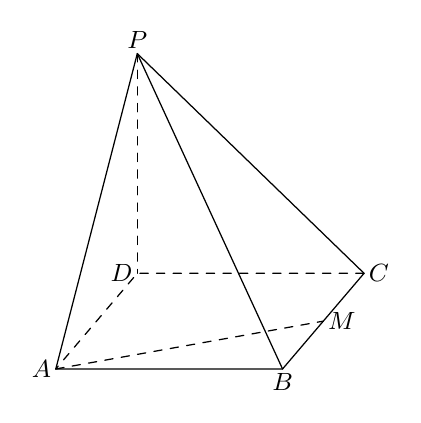
\begin{tikzpicture}[
  x=0.9cm, y=0.9cm,
  font=\small,
  line width=0.45pt,
  line cap=round,
  line join=round,
  every node/.style={inner sep=1.5pt}
]
  \coordinate (A) at (0,0);
  \coordinate (B) at (3.2,0);
  \coordinate (C) at (4.35,1.35);
  \coordinate (D) at (1.15,1.35);
  \coordinate (P) at (1.15,4.45);
  \coordinate (M) at (3.775,0.675);

  % 锥面棱。
  \draw (P) -- (A);
  \draw (P) -- (B);
  \draw (P) -- (C);
  \draw[dashed] (P) -- (D);

  % 矩形底面。
  \draw (A) -- (B) -- (C);
  \draw[dashed] (C) -- (D) -- (A);

  % 题设辅助线 AM。
  \draw[dashed] (A) -- (M);

  \node[anchor=east] at (A) {$A$};
  \node[anchor=north] at (B) {$B$};
  \node[anchor=west] at (C) {$C$};
  \node[anchor=east] at (D) {$D$};
  \node[anchor=south] at (P) {$P$};
  \node[anchor=west] at (M) {$M$};
\end{tikzpicture}
\end{center}
\nopagebreak[4]
(1) 证明：平面 $PAM\perp$ 平面 $PBD$；

(2) 若 $PD=DC=1$，求四棱锥 $P-ABCD$ 的体积。

\end{question}
\begin{question}
\gkti{19}设 $\{a_n\}$ 是首项为 $1$ 的等比数列，数列 $\{b_n\}$ 满足 $b_n=\dfrac{na_n}{3}$。已知 $a_1,3a_2,9a_3$ 成等差数列。

(1) 求 $\{a_n\}$ 和 $\{b_n\}$ 的通项公式；

(2) 记 $S_n$ 和 $T_n$ 分别为 $\{a_n\}$ 和 $\{b_n\}$ 的前 $n$ 项和，证明 $T_n<\dfrac{S_n}{2}$。

\Needspace{0.4\textheight}

\end{question}
\begin{question}
\gkti{20}已知抛物线 $C:y^2=2px\ (p>0)$ 的焦点 $F$ 到准线的距离为 $2$。

(1) 求 $C$ 的方程；

(2) 已知 $O$ 为坐标原点，点 $P$ 在 $C$ 上，点 $Q$ 满足 $\overrightarrow{PQ}=9\overrightarrow{QF}$，求直线 $OQ$ 斜率的最大值。

\end{question}
\begin{question}
\gkti{21}设函数 $f(x)=x^3-x^2+ax+1$。

(1) 讨论 $f(x)$ 的单调性；

(2) 求曲线 $y=f(x)$ 过坐标原点的切线与曲线 $y=f(x)$ 的公共点的坐标。

\end{question}
\begin{question}
\gkti{22}在直角坐标系 $xOy$ 中，$\odot C$ 的圆心为 $C(2,1)$，半径为 $1$。

(1) 写出 $\odot C$ 的一个参数方程；

(2) 过点 $F(4,1)$ 作 $\odot C$ 的两条切线，以坐标原点为极点，$x$ 轴正半轴为极轴建立极坐标系，求这两条切线的极坐标方程。

\end{question}
\begin{question}
\gkti{23}已知函数 $f(x)=|x-a|+|x+3|$。

(1) 当 $a=1$ 时，求不等式 $f(x)\geqslant6$ 的解集；

(2) 若 $f(x)>-a$，求 $a$ 的取值范围。

\makeatletter\def\gkanswerblock{answer}\ifx\@currenvir\gkanswerblock\else\clearpage\fi\makeatother

\end{question}